Since experiments in biology usually involve a comparison of multiple samples, it is necessary to align the LC-MS data (produced from multiple samples) in order to compare them. We define a single result from running a sample through the LC-MS machine to be a \noun{replicate}. Once replicates have been produced in a metabolomic experiment, they need to be aligned. Alignment methods attempt to match peaks in correspondence across replicates. This is usually done by finding the mapping function that maps the retention time from one replicate to another. To produce a more robust method of aligning peaks, it is important to understand the characteristics of existing alignment methods. In this chapter, we first outline the current challenges in performing alignments of label-free LC-MS data. Next, two broad types of alignment methods are compared and constrasted: profile-based and feature-based alignment methods.

\subsection{\label{sec:Challenges-in-Peak}Challenges in Peak Alignment of Label-Free
Experiments}

% Label-free experiments pose many challenges in analysing replicates from different LC-MS runs. In particular, peaks from different runs can experience a potentially non-linear shift in retention time across chromatograms \cite{Podwojski2009}. There is often a large amount of variations in the retention times across the replicates. Retention time variation could be due to instrument-specific factors (the condition of the chromatographic column itself. including flow rate variations, gradient slope and temperature \cite{Christin2008}) or experiment-specific factors (e.g. instrument malfunctions or columns that need be replaced mid-experiment). Both factors are difficult to control, even in a careful experimental setting. Consequently, a single peak from one replicate can have several potential matches peaks in another replicate. This can also introduce false positives into the alignment result As a result, \emph{replicates produced by different LC-MS platforms or from different laboratories cannot be easily aligned to each other}. In particular, the non-linear variation in retention time makes aligning technical replicates (which contains the same composition of metabolites) difficult and aligning biological replicates (which may not contain the same composition of metabolites) even more challenging.

% Since large-scale untargeted metabolomics study can generate a huge number of samples (see \cite{DeVos2007a,Creek2011}), having a reliable and accurate peak alignment step during data preprocessing is important. Peaks that are improperly aligned can lead to false positives. Especially for label-free untargeted metabolomic experiments, the presence of even relatively small errors in any steps preceding the identification stage (including alignment) can result in significant differences to the final analysis and biological conclusions. Errors or uncertainties inadvertently produced in any sub-step before identification would be carried forward forward in the pipeline. Improper preprocessing steps can also introduce variabilities that obscure important biological variations of metabolites themselves \cite{Katajamaa2007}. Having a robust alignment method that can align a large number of replicates with high precision is therefore an important research question to be addressed.

% Additionally, it is also desirable for alignment methods to provide some measure of confidence in the quality of its alignment. In the absence of ground truth information, life scientists typically measures alignment quality through manual inspection or by comparing and visualising the summary statistics (e.g. median, standard deviation of retention time) across different replicates. Alignment methods with confidence values is a big research gap that, to our knowledge, has not been addressed at all by any of the alignment tools surveyed earlier. Some interactive analysis tools like MAVEN \cite{Melamud2010} can assign quality scores to individual peaks. This is accomplished by training a neural network (or a decision tree) on training data that have been manually annotated using metrics of peak quality. Other approach like \cite{Brodsky2010} computes the Pearson correlations between intensity profiles of all peaks across replicates. Moving from these approaches towards a robust method that can provide confidence values for groups of aligned peaks across many label-free experiments is challenging research problem.

\subsection{\label{sub:Approaches-in-Peak}A Survey of Alignment Methods}

% Broadly speaking, the main challenge in peak alignment is caused by the poor reproducibility of retention time, with large non-linear shifts and distortions across replicates (see \ref{fig:We-plot-the} for example) . Consequently, most alignment methods correct for those shifts and distortions by finding -- either explicitly or implicitly -- a mapping function $f$ that maps time $t$ in one replicate to $f(t)$ in another. The mapping function $f$ should be a monotonically smooth and increasing function, since elution orders of peaks that come out from the liquid chromatography instrument are generally preserved across replicates (at least for data produced from the same LC-MS instruments). The main differences come from whether the alignment method operates on the entire raw LC-MS data (profile-based method) or on a reduced set of features extracted from the data (feature-based method).

\begin{figure}[h]
\noindent \begin{centering}
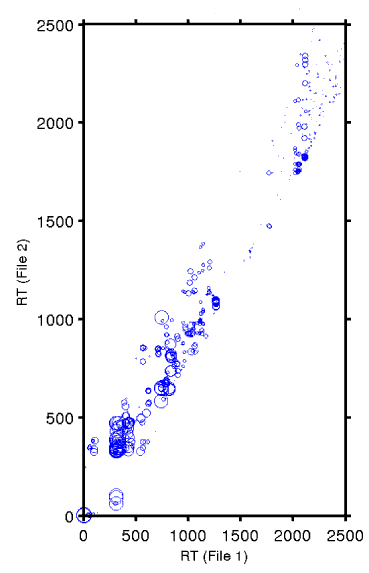
\includegraphics[width=0.5\textwidth]{images/nonlinear2}
\par\end{centering}

\caption{\label{fig:We-plot-the}We plot the retention time of matching peaks from two replicates produced from real LC-MS experiments. Peaks are scaled in the plot based on a putative confidence score in the quality of their alignments. We can see that aligned peaks exhibit non-linear shifts in their retention time across the two replicates. Matching peaks across replicates and finding the mapping function $f$ that maps time $t$ in one replicate to $f(t)$ in another are therefore hard problems.}

\end{figure}

\subsubsection{\label{sub:Profile-based-Alignment-Methods}Profile-based Alignment
Methods}

The profile-based method aligns the whole ion chromatograms (profile data) directly, usually by mapping the retention time axes from one profile to another. Since the alignment step is performed before peak detection, profile-based methods do not depend on the correctness of detected peaks. In profile-based alignments, the profile data being aligned is reduced to a simpler form by summing together the intensity values over the whole range of mass values. This produces either the total ion chromatograms (TIC) \footnote{The total ion chromatogram is the sum of all intensities across the whole range of masses in the LC-MS profile} when all peaks in each mass spectrum are considered, or the base peak chromatograms \footnote{The base peak chromatogram is like the TIC, but using only the most intense peak in each mass spectra} when only the most intense peak in each mass spectrum is considered (\ref{fig:profile-based}).

\begin{figure}[h]
\noindent \begin{centering}
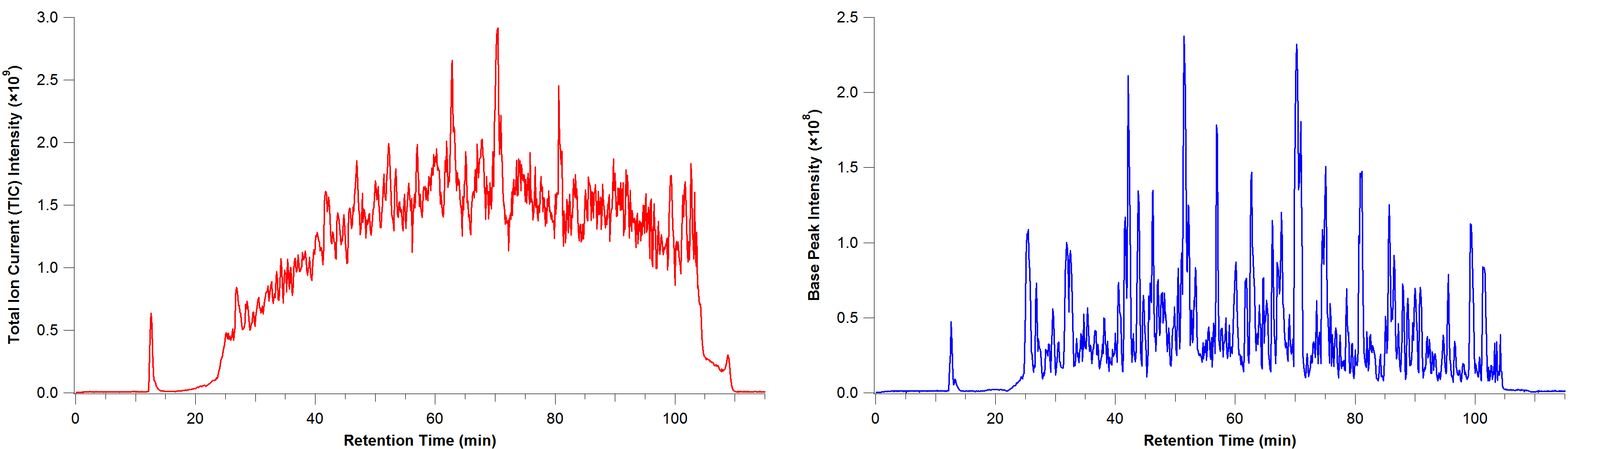
\includegraphics[width=1\textwidth]{images/tic_base_peaks}
\par\end{centering}

\caption{\emph{\label{fig:profile-based}}The raw LC-MS profile data is often reduced to a simpler form for profile-based alignments. The total ion chromatogram (TIC) is the sum of all intensities across the whole range of masses in the LC-MS profile (left figure). If only the most intense peak is considered when summing over the whole range of masses, the base peak chromatograms are obtained (right figure). However, information on the mass dimension in the profile data is lost due to the summing. Profile-based alignment methods find the retention time mapping function $f$ between replicates by aligning multiple TIC or base peak chromatograms.} \end{figure}

Dynamic programming algorithms are commonly used in profile-based alignments. In dynamic programming, all possible local solutions are evaluated but computed only for each sub-problem. In theory, this allows for an optimal global solution to be obtained efficiently. In practice, exact dynamic programming solutions are often intractable when many replicates need to be aligned at once. Some examples of profile-based alignment methods are highlighted here:

\begin{description}

\item [{Dynamic~Time~Warping~(DTW)~\cite{Sakoe1978,Tomasi2004}}] For pairwise alignment using DTW, the total ion chromatograms or the base peak chromatograms being aligned are first discretised along the RT axes. Finding the alignment path is accomplished by setting up an alignment matrix and obtaining the best warping path that minimises the global distance in the alignment matrix. Three weight factors that computes the penalty for matches, expansion and compression are defined. The optimal warping path is obtained by applying dynamic programming principle and tabulating intermediate results in the alignment matrix (in a manner similar to global sequence alignment for DNA sequences). The best warping path can then be read by backtracking from the final entry of the alignment matrix to the start.

\item [{Correlation~Optimised~Wrapping~(COW)~\cite{Nielsen1998,Tomasi2004}}] Similar to DTW, COW also operates on the discretised total ion/base peak chromatograms. COW divides the RT axes of replicates into segments. Each segment boundary can change within some user-specified slack parameter. COW then produces an alignment by finding the path across segments that has the highest sum of correlations. An alignment matrix is set up, and different segment boundaries can be shifted to maximise the global correlations between the two replicates being aligned using dynamic programming. Christin, et al. (2008) \cite{Christin2008} combines COW with a component detection algorithm (CODA \cite{Windig1996,Windig2007}) that removes noisy signal and background noise from the mass chromatograms, aligning only 'regions containing high-quality information'.

\item [{Parametric~Time~Warping~(PTW)~\cite{VanNederkassel2006}}] Parametric Time Warping (PTW) produces pairwise alignment by using a second degree polynomial for mapping time between chromatograms. Coefficients of the polynomial are optimised by minimising the sum of squared residuals between the reference and aligned chromatograms. PTW performs much faster than COW. However, the quadratic polynomial model proposed in PTW, while simpler to describe, might not be sufficient to capture the complexity in non-linear retention time drifts across LC-MS data \cite{Podwojski2009}. Semi-parametric Time Warping (STW) extends upon PTW and uses a series of B-splines as the mapping function. Optimising the warping coefficients in STW is done iteratively.

\item [{Continuous~Profile~Mode~(CPM)}] Listgarten, et al. \cite{Listgarten2005} proposed a generative Continuous Profile Model (CPM) for aligning multiple LC-MS data in a time series using a hidden Markov model-based approach. Each observed chromatogram profile is considered to be a time series of noisy signals sampled from a canonical latent profile. Parameters of the model are trained using the Expectation-Maximisation algorithm. The actual alignment of observed profiles to the latent profile is done using Viterbi algorithm. Compared to previous pair-wise methods such as DTW, CPM alignment is more robust since it aligns multiple LC-MS data simultaneously. As a common advantage for profile-based alignments, potential errors are minimised by combining the peak detection and alignment step into one.

\end{description}

All the profile-based alignment methods surveyed above performs alignment using only the total-ion chromatograms or the base peak chromatograms\emph{, }this ignores the rich information present in the mass dimension of LC-MS data. As a consequence, such profile-based methods might not perform as well for alignments of typical LC-MS data produced from complex mixtures -- frequently having a lot of peaks of different m/z values co-eluting at similar retention times. Furthermore, profile-based methods also do not generalise well to aligning multiple LC-MS profiles in more than 2 replicates. Since dynamic programming approach has a high time complexity when aligning multiple profile data simultanously, many of the profile-based alignments surveyed above aligns replicates in a hierarchical pairwise manner. This might fail to consider potential systematic variations that are present across multiple datasets, which is necessary when aligning biological replicates (as opposed to just aligning technical replicates).

Since untargeted metabolomic experiments often produce a large number of replicates, all of which need to be aligned as correctly as possible, most of the recent advances in alignment are based on aligning 'features', a reduced representation of the raw LC-MS data.

\subsubsection{\label{sub:Feature-based-Alignment-Methods}Feature-based Alignment
Methods}

A feature is a representation of signal that have been extracted from the raw ion chromatograms. It usually consists of essential information such as the mass-to-charge ratios (m/z), retention times and intensities values extracted from the signal (peak). In this manner, we can define a feature to be a a vector of its mass, time and intensity values
$p_{i}=\left(\begin{array}{c}
mass\\
time\\
intensity
\end{array}\right)$. A replicate $R$ is therefore a set of distinct features $R=\{p_{1},p_{2},...,p_{n}\}$. The pairwise alignment problem reduces to matching features from one replicate $R_{i}$ to another replicates $R_{j}$, through any of the methods outlined below. The problem can also be generalised to alignments of multiple replicates. We can see that on top of finding the mapping function $f$ that maps retention time from one replicate to another, feature-based alignment methods also encompass peak matching, i.e. finding the correspondence of peaks that come from the same metabolite from one sample to another.

\begin{figure}[h]
\noindent \begin{centering}
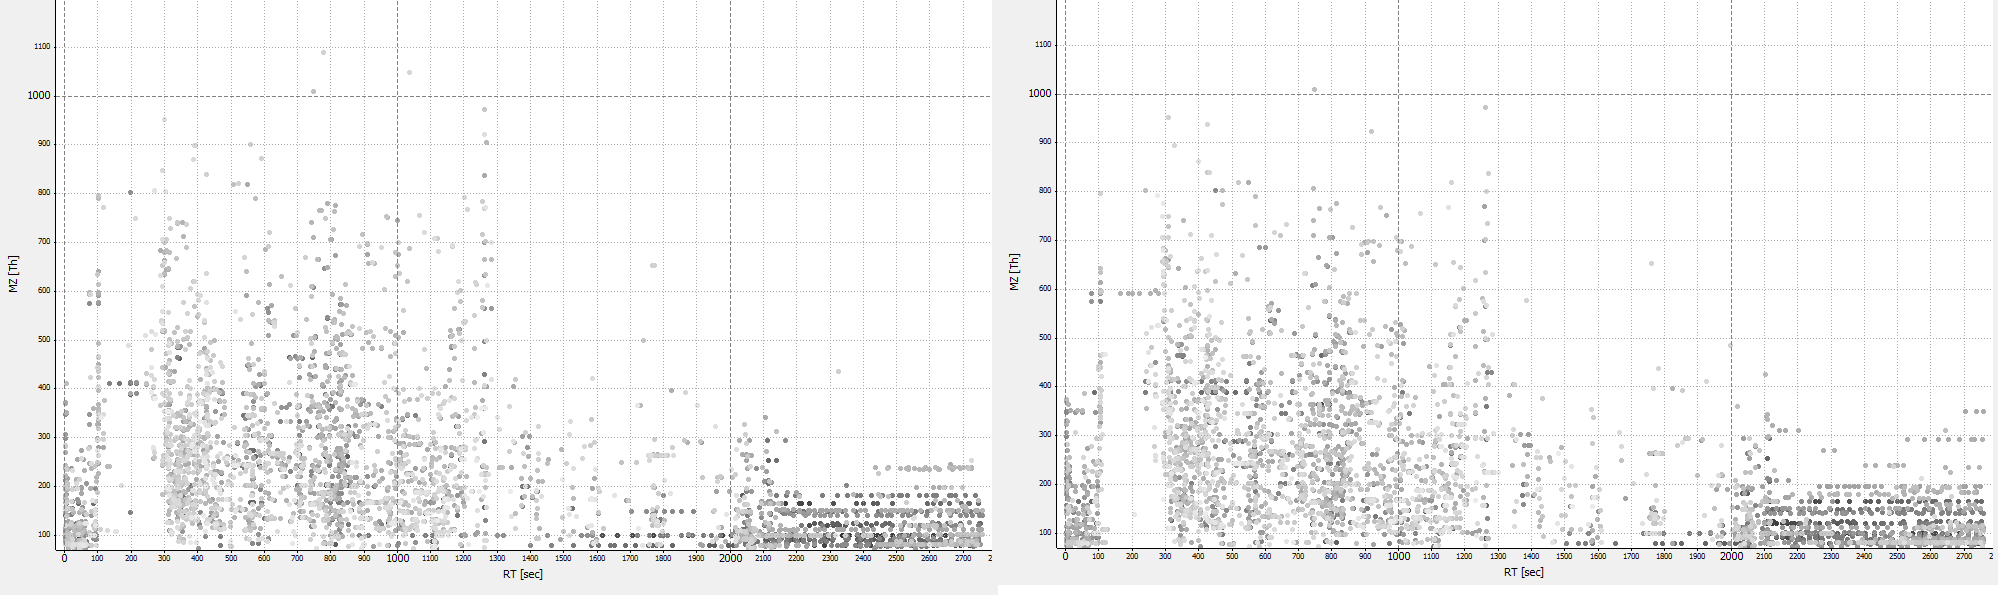
\includegraphics[width=1\textwidth]{images/feature}
\par\end{centering}
\caption{\emph{\label{fig:feature-based}}Peak detection step can identify features (peak) from the raw LC-MS profile data. The term 'feature' and 'peak' are often used interchangeably in feature-based alignments. A feature is a vector of m/z, intensity and retention time. In this figure, each dot is a detected feature. Darker dots have higher intensities. The two replicates shown here have minimal noise to the retention time, so finding the correspondence between features across the two replicates are fairly simple. Alignment becomes much harder when non-linear drifts in the retention time occurs from one replicate to another.}
\end{figure}

Many of the recent LC-MS data preprocessing tools surveyed perform feature-based alignment, because the raw LC-MS data is complex and difficult to align correctly -- particularly when many replicates are produced during the experiment (as explained previously). Feature-based approaches makes it easier to incorporate mass, intensities and other structural information that can potentially help improve the alignment result. By extracting a smaller set of features from complex LC-MS raw data, it is also easier and faster to align many replicates at once. From the various feature-based methods surveyed, we can identify three major strategies employed by feature-based alignment methods, namely: greedy alignment methods, curve-fitting alignment methods and combinatorial alignment methods.

Greedy algorithm works by making a locally optimal choice at each step of its processing with the hope that this will lead to a globally optimal solution in the end \cite{Cormen2009}. The typical greedy approach works by iterating through the features in some reference list, successively aligning each feature against other features in different replicates. The retention mapping function $f$ is implicitly discovered through successful matching of sets of features that are 'close' enough, usually based on maximising some scoring function or minimising an overall distance measure.

Because of its simplicity, it is often the default go-to method for feature-based alignments in some LC-MS data preprocessing toolkit.
Some examples of recent greedy alignment methods are highlighted here:

\begin{description}

\item [{mzMatch~\cite{Scheltema2011}}] The mzMatch toolkit that has been under development inside the University of Glasgow for processing of LC-MS data employs this greedy approach towards alignment. In mzMatch alignment, all features are first sorted by their intensities in descending order. mzMatch aligns the first (unaligned) feature having the highest intensity to other features in other replicates that fall within a mass tolerance and having sufficiently close distance in mass and retention time tolerance. The mass tolerance -- expressed in units of ppm parts-per-million -- is specified by the user and usually depends on the accuracy of mass spectrometer. mzMatch computes the distance between two features by some fairly ad-hoc heuristics: checking that their retention time fall within user-defined tolerance and comparing the area under the curve of their signals.

\item [{MZmine's~Join~Aligner~\cite{Pluskal2010}}] Another toolkit that is commonly used for LC-MS data processing is MZmine. The Join Aligner in MZmine operates in a greedy manner: an initial empty master list is created. Subsequent feature lists are aligned against this master list. A feature entry in the currently processed list is merged to an existing entry in the master list if the feature's score is within mass and retention time tolerances. Otherwise it is appended as a new entry in the master list. This process is repeated iteratively until all feature lists have been processed, progresively 'joining' a feature list to the master list. This alignment approach is an instance of a greedy algorithm, where locally optimal choice is made in each stage (here, by joining a feature against matching rows in the master list) in the hope that a globally optimum solution is reached. Join Aligner has been chosen for inclusion into our evaluation pipeline, and is described more in \ref{sub:Join-Alignment}.

\end{description}

\subsubsection{Curve-fitting Alignment Methods}

To deal with the non-linear nature of retention time shifts in LC-MS data, another common approach is to attempt to fit a curve based on the training data available. These are usually all the features observed across replicates or some selected subsets of all features observed. The retention time drifts of observed features from one replicate to another are then modelled by the mapping function $f$, which is usually obtained through nonlinear regressions. Some curve-fitting tools also finds the time mapping function $f$ but do not perform feature matching. This requires an additional step of performing the actual feature matching to find the correspondence of features derived from the same metabolites across different replicates.

Some examples of recent curve-fitting alignment methods are highlighted
here:

\begin{description}

\item [{XCMS~\cite{Smith2006}}] XCMS is one of the oldest tool used in metabolomics for processing mass spectrometry data and metabolite profiling. Alignment is XCMS is performed in two stages: peak matching \& retention time correction. During the peak matching stage, the m/z axis is divided into discrete fixed-width overlapping bins. The alignment algorithm constructs a Gaussian kernel density estimation of the peaks inside each bin. This results in groups of peaks ('meta-peaks') that are close in their masses. Groups that do not contain enough peaks across samples are discarded. Next, during the retention time correction stage, well-behaved groups are selected as landmark peaks. The median retention time of each group is calculated, and the deviation from the median for each peak is used to train a local regression model. The resulting regression is used to correct for peak deviations.

\item [{OpenMS~\cite{Lange2007}}] OpenMS alignment works by first selecting a replicate that has the highest number of features. This replicate is used as the reference replicate, against which all other replicates are aligned against (in a star-like manner). The actual alignment process is divided into following two phases: superposition and consensus. During the superposition phase, the alignment algorithm tries to find the parameter for an affine transformation that maximises the number of features mapped from the reference replicate to the other replicates. An object recognition algorithm, called pose clustering, is used for this purpose. Additional information -- such as m/z, RT and intensity dimension -- is considered during the clustering process. The subsequent consensus phase then produces the actual alignment between matching features across replicates, using nearest-neighbour criteria. In the evaluation by Lange, et al. \cite{Lange2008}, the OpenMS alignment performs best for aligning replicates that are produced over a course of different days and having large retention time drift.

\item [{MZmine's~RANSAC~Aligner~\cite{Pluskal2010}}] Pluskal, et al. further proposes an improved alignment algorithm based on Random Sample Consensus (RANSAC) that addresses the weakness of the Join aligner in dealing with the non-linear variations in retention time across samples. The RANSAC algorithm has a user-defined mass and retention time tolerance parameters, which are used to select features for training a local regression model. The model is used for correcting the retention time drifts of features across aligned samples. The RANSAC Aligner has been chosen for inclusion into our evaluation pipeline, and is described more in \ref{sub:RANSAC-Alignment}.

\end{description}

\subsubsection{Combinatorial Alignment Methods}

From literature survey, recent advances in feature-based alignment treats feature-based alignments as a combinatorial optimisation problem. This is accomplished by defining an objective function that minimises the difference between aligned features (usually by the difference in their masses and retention times). Alignment between features are then obtained by finding the matching of features that maximise this objective function. Pairwise alignment between 2 replicates are found using algorithms that solve for the stable marriage problem, while alignments between multiple replicates can found using algorithms that solve for the maximum weight matching problem in a general graph.

Some examples of recent optimisation-based alignment methods are highlighted
here:

\begin{description}

\item [{SIMA~\cite{Voss2011a}}] SIMA (SImultaneous Multiple Alignment) defines a custom Mahalanobis distance for feature similarity. The distance is used for ranking feature's preferences in finding a stable matching between replicates using the Gale-Shapley algorithm for stable matching. Instead of using a fixed reference replicate to align to, SIMA chooses the pairing of replicates to align in a hierarchical order. Replicates are greedily aligned based on their overall similarity of features, with the closest replicates aligned first. An additional step to estimate the retention time mapping function $f$ using ridge regression is also provided to implicitly correct for the non-linear time shifts, although such step is optional and not required to obtain the alignment result. SIMA has been chosen for inclusion into our evaluation pipeline, and is described more in \ref{sub:SIMA}.

\item [{BIPACE~\cite{Hoffmann2012a}}] BIPACE (BIdirectional best hits Peak Assignment and Cluster Extension) defines a cosine similarity function between features. All pairwise similarities between features in K replicates are then computed. A K-partite graph G is created, where each replicate defines a disjoint partition of features in the graph and the edges are the pairwise similarity between the features. Several heuristic rules are then applied to G to reduce the complexity of the graph by pruning 1) edges between features that are outside the retention time tolerance of each other, and 2) vertices that are not closest in similarity ('bidirectional best hits') from each other. Finally, greedy merging are performed to enumerate all maximal cliques in the graph. All cliques above some user-defined threshold essentially form the alignment between features. Similar to SIMA, an additional step to estimate the retention time mapping function $f$ is also possible, using a dynamic time-warping approach (see section \ref{sub:Profile-based-Alignment-Methods}).

\item [{SMFM~\cite{Lin2013}}] SMFM (Suboptimal Maximum Feature Matching) produces an optimal solution to the maximum matching problem by relaxing the bijective mapping requirement, assuming that one feature in a replicate can be matched to multiple other features in another replicate (surjective mapping). This relaxation allows SMFM to establish an upper bound to the maximum weight of features under surjective mapping and also compute the optimal retention time mapping function $f$ under such a relaxed case. The actual extraction of alignment is performed by computing a maximum bipartite matching, but using the optimal time mapping function $f$ obtained under surjective mapping. An extension to allow for gapped alignment is also provided.

\end{description}

\subsection{Performance Evaluation of Alignment Methods}

Performance evaluation of data pre-processing algorithms in metabolomics is difficult due to the lack of gold standard and evaluation criteria for benchmarking \cite{Castillo2011}. Among all the alignment methods surveyed earlier, we found a wide range of approaches towards evaluating the quality of alignment result. In \cite{VanNederkassel2006}, three profile-based tools (COW, PTW and STW) were compared. Evaluation of alignment quality was performed through manual visual inspection of superimposed profile images and some selected chromatograms. This visual comparison was also used for evaluating the performance of CPM in \cite{Listgarten2005}. While straightforward, visual inspection of alignment quality is not a systematic approach towards performance evaluation, since visual inspection is often subjective and might suffer from dissimilar interpretations across different experiments and datasets.

\textbf{Another common way to evaluate profile-based alignment is
to compute RT/CV difference, and to see how it improves peak matching
\cite{Tsai2013a}}

The situation is better for feature-based alignments. Lange, et al. \cite{Lange2008} introduced a set of LC-MS data that have their associated alignment ground truth. This dataset can be used as the gold standard for benchmarking feature-based alignment tools in proteomics and metabolomics. The dataset has been integrated into our evaluation pipeline and described in greater details in \ref{sub:Evaluation-Data-Source}. Most of the feature-based alignment tools described earlier (including MZmine, XCMS, OpenMS and SIMA) have been evaluated on this Benchmarking dataset. Using a common dataset for performance evaluation allows for meaningful comparisons of alignment tools. However, this is only as good as the quality of ground truth produced by Lange, et al. In \ref{sub:Performance-Evaluation}, we describe in more details how precision and recall are calculated for the Benchmarking dataset. In particular, we note that not all features in a replicate are included in the ground truth. From our observation, approximately only one-fifth of all features in a replicate have their corresponding alignment ground truth entries for the metabolomics data (M1 \& M2).

On top of using the Benchmarking dataset, most of the feature-based alignment tools surveyed earlier also evaluate their performance on a simulated dataset. Performance of individual tools on simulated data are often very good. Simulated data might be constructed in such a way that favours the new tool being developed. For example, MZMine's RANSAC Aligner \cite{Pluskal2010} obtains a perfect precision (1.0) and recall (1.0) when evaluated using the simulated data that they have constructed. For evaluation using simulated data to be effective, there needs to be a common LC-MS simulator that can generate synthetic feature data to be aligned by various alignment tools under different noisy conditions. Such a simulator can then be used to provide an objective context for comparing the performance of future LC-MS alignment tools using simulated data. This is addressed as a potential future work in \ref{sec:Alignment-using-Simulated}.

Lastly, some alignment tools also evaluate their performance by computing various summary statistics, such as the average aligned retention time errors, the mean standard deviations of retention time, and the percentage of correctly aligned feature pairs (for example, in \cite{Lin2013,Podwojski2009}). Computing summary statistics provide a global single value to represent retention time quality. This often fails to take into account the trade-off between precision and recall. For example, an alignment method can match only pairwise features having low absolute retention time error and discards everything else. This tool will have a minimal retention time error. However, the resulting alignment will not be considered good in practice. It is often preferred to use the more established concepts of precision and recall for performance evaluation of alignment result.

\subsection{Summary}

In this section, we have surveyed the two common approaches in performing alignment: profile-based and feature-based methods.

Profile-based methods can potentially take into account \emph{all the available information available in the raw LC-MS data.} Despite the availability of information in the raw profile data, most profile-based methods surveyed so far aligns peaks using only on their retention time information. Incorporating additional information into the alignment process, for example through a dynamic programming method that seeks for an optimal solution in the mass and retention time dimensions, is often too expensive to be practical.

While profile-based method is not sensitive to the potential errors from the preceding peak detection stage, most profile-based methods usually take a long time to run and do not perform well for aligning multiple replicates at once. More importantly, the profile-based methods surveyed usually have a large number of parameters to tune to produce a good alignment result. Typical users from a life-science background are often at lost to the intricacies of tuning these parameters to produce good results. For all these reasons, profile-based methods seem to be falling out of favour -- with most of the recent advances in alignment occuring from a feature-based perspective. For this reason, I will generally adopt a feature-based approach for the remaining work in this PhD (although extending it to profile-based methods remains an open possibility).

The many feature-based approaches surveyed so far can be broadly divided into three classes: greedy algorithms, curve fitting algorithms and combinatorial algorithms. Because of its simplicity (from an algorithmic development point of view), greedy algorithms are quite widely used as an initial attempt towards performing alignments in many metabolomics toolkit. With the selection of appropriate heuristics, greedy algorithms can indeed produce a 'good enough' solution for some users. However, the greedy approach has been found to be lacking when aligning LC-MS data with non-linear shift in retention time across replicates. In contrast, curve-fitting algorithms, employing non-linear regression models, is more suitable for this situation. In practical use however, curve-fitting algorithms can be dauntingly complex to use by typical life scientists. Small changes to the parameters of the models might produce substantially different results. This situation generally applies to any complex regression models.

The final class of feature-based alignment method surveyed is combinatorial algorithms. The problem of peak matching naturally fits well with combinatorial approaches for solving the problem of matching under preference. A stable solution to bipartite matching between two replicates can be found using well-established algorithm, such as the Gale-Shapley algorithm, with quadratic time complexity. The solution obtained from Gale-Shapley is stable but might not be optimal. Performance evaluation for SIMA, which employs the Gale-Shapley algorithm for stable matching, was found to be superior to other greedy and curve-fitting alignment tools. From literature surveyed, combinatorial approaches also contribute to most recent advances in feature-based alignments.

Finally, we have also explained how performance evaluation of alignment result is an open problem. Evaluating alignment result through visual inspections or by computing various summary statistics should be taken with care. The availability of the Benchmarking data and having a common LC-MS simulator are useful in providing a fair and objective way to compare the performance of feature-based alignment tools .
